\listfiles
\RequirePackage{rotating}
\documentclass[manuscript, review, screen, authordraft]{acmart}

% bibliography
% using biblatex isn't very smart because journals are pretty picky. Instead use the default natbib package
% \usepackage[backend=biber,style=trad-abbrv]{biblatex}
% \addbibresource{References.bib}

%\setcitestyle{super,sort&compress}
% \citestyle{acmauthoryear}
\usepackage{booktabs} % For formal tables

\usepackage[ruled]{algorithm2e} % For algorithms
\usepackage{subcaption}

% Metadata Information
\acmJournal{CSUR}
\acmVolume{VV}
\acmNumber{NN}
\acmArticle{AA}
\acmYear{YYYY}
\acmMonth{MM}

%\acmBadgeL[http://ctuning.org/ae/ppopp2016.html]{ae-logo}
\acmBadgeR[http://ctuning.org/ae/ppopp2016.html]{ae-logo}

% Copyright
% \setcopyright{acmcopyright}
%\setcopyright{acmlicensed}
\setcopyright{rightsretained}
%\setcopyright{usgov}
%\setcopyright{usgovmixed}
%\setcopyright{cagov}
%\setcopyright{cagovmixed}

% DOI
\acmDOI{0000001.0000001}

% some useful shortcut commands
\newcommand{\Pl}{\textbf{Pl}}
\newcommand{\R}{\textbf{R}}

% Document starts
\begin{document}
% Title portion
\title{``I can assure you [\ldots] that it's going to be all right''} 
 \titlenote{HAL, 2001 A Space Odyssey, full quote: ``I know everything hasn't been quite right with me, but I can assure you now, very confidently, that it's going to be all right again.''}
 \subtitle{A definition, case for, and survey of algorithmic assurances in human-autonomy trust relationships}
 \subtitlenote{Subtitle note}
\author{Brett Israelsen}
    \authornote{The corresponding author}
    \orcid{0000-0003-1602-1685}
    \email{brett.israelsen@colorado.edu}
    \affiliation{%
        \institution{University of Colorado, Boulder}
        \institution{Department of Computer Science}
        \city{Boulder}
        \country{USA}
    }
    \affiliation{%
        \institution{RECUV}
    }
    \affiliation{%
        \institution{C-UAS}
    }

\begin{abstract}
    I need to add an abstract here. I think it will include things about the pervasive need across multiple disciplines to understand and quantify the functions of AIs. I will try to talk about different research areas and outline each of their needs and some of the methods that they currently  use. I hope to be able to identify several places for opportunity, and possibly introduce some fields to others.
\end{abstract}


%
% The code below should be generated by the tool at
% http://dl.acm.org/ccs.cfm
% Please copy and paste the code instead of the example below. 
%
\begin{CCSXML}
<ccs2012>
 <concept>
  <concept_id>10010520.10010553.10010562</concept_id>
  <concept_desc>Computer systems organization~Embedded systems</concept_desc>
  <concept_significance>500</concept_significance>
 </concept>
 <concept>
  <concept_id>10010520.10010575.10010755</concept_id>
  <concept_desc>Computer systems organization~Redundancy</concept_desc>
  <concept_significance>300</concept_significance>
 </concept>
 <concept>
  <concept_id>10010520.10010553.10010554</concept_id>
  <concept_desc>Computer systems organization~Robotics</concept_desc>
  <concept_significance>100</concept_significance>
 </concept>
 <concept>
  <concept_id>10003033.10003083.10003095</concept_id>
  <concept_desc>Networks~Network reliability</concept_desc>
  <concept_significance>100</concept_significance>
 </concept>
</ccs2012>  
\end{CCSXML}

\ccsdesc[500]{Computer systems organization~Embedded systems}
\ccsdesc[300]{Computer systems organization~Redundancy}
\ccsdesc{Computer systems organization~Robotics}
\ccsdesc[100]{Networks~Network reliability}

%
% End generated code
%

% We no longer use \terms command
\terms{Design, Algorithms, Performance}

\keywords{Wireless sensor networks, media access control,
multi-channel, radio interference, time synchronization}


\thanks{This work is supported by C-UAS.}

  % Author's addresses: G. Zhou, Computer Science Department, College of
  % William and Mary; Y. Wu {and} J. A. Stankovic, Computer Science
  % Department, University of Virginia; T. Yan, Eaton Innovation Center;
  % T. He, Computer Science Department, University of Minnesota; C.
  % Huang, Google; T. F. Abdelzaher, (Current address) NASA Ames
  % Research Center, Moffett Field, California 94035.}

\maketitle

\section{Introduction}
    As technology becomes more advanced those who design, use, and are affected by it in other ways want to know that it will perform correctly, and understand why it does what is does, and how to use it appropriately. In essence people who interact with advanced technology want to be able to trust it appropriately, and then act on that trust.

    Specifically, in this survey, I investigate what assurances an Artificially Inteligent Agent (AIA) can provide to a human user in order to affect their trust. The terms `appropriate use`, `assurance`, `AIA`, and `trust` will be further defined later in the paper; for now the common definitions should suffice to give the reader a general idea of the motivation.

    Some examples of AIAs include an image classifier, a credit approval algorithm, a personal assistant software, a recommender system, a self-driving vehicle, and many others.

    In interpersonal relationships and otherwise humans act based on trust. For example a supervisor asks a subordinate to accomplish based on several factors that indicate they can trust them to accomplish the task. When consumers make purchases they do so with trust that the product will perform to the promised specifications. Likewise, when using something like an autonomous vehicle the user must be able to trust it appropriately in order to use it properly. \textbf{I really don't like this paragraph much, but I'll have to come back later}.

    That then begs the question: what can an AIA do in order to ensure that a user trusts it appropriately, and will therefore *use* it appropriately?

    \begin{figure}
        \centering
        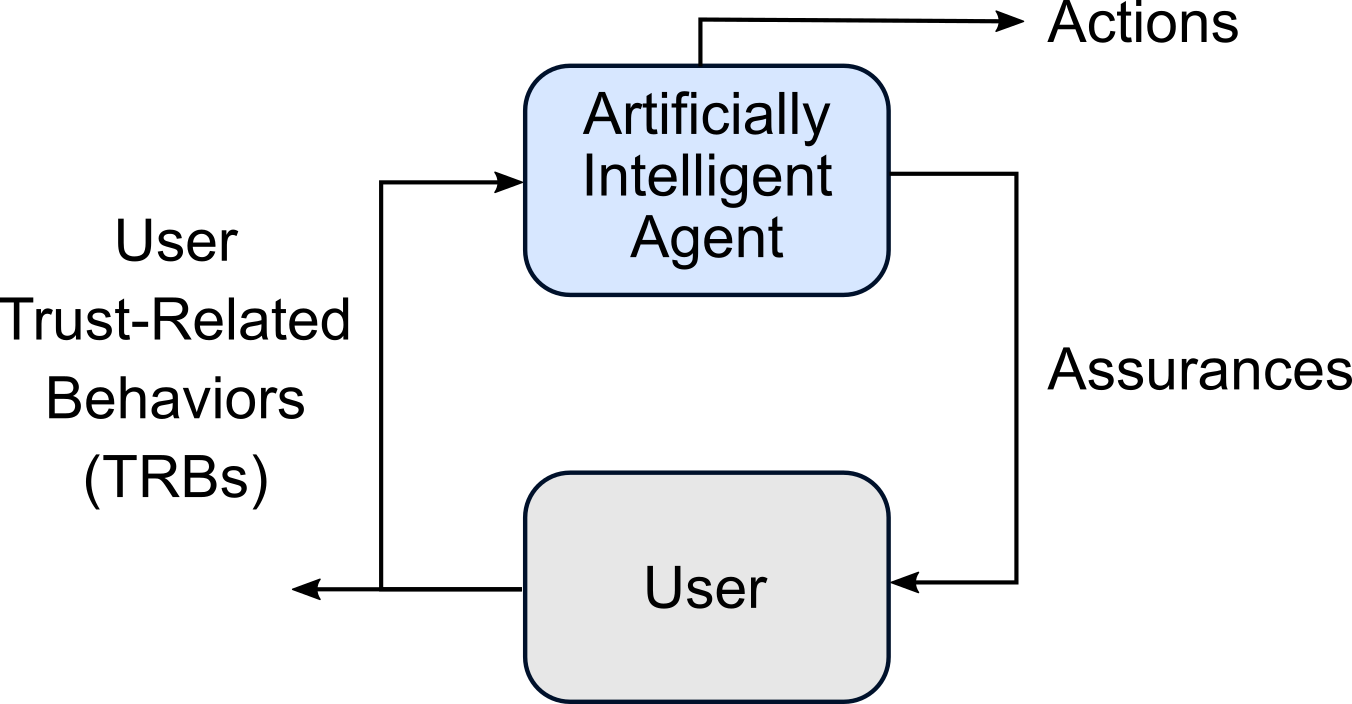
\includegraphics[width=0.5\textwidth]{Figures/SimpleTrust_one_way.png}
        \caption{stuff}
    \end{figure}

\subsection{Artifically Intelligent Agents}
    An Artificial General Intelligence (AGI) would possess at least the capabilities shown in Figure \ref{fig:AIcapabilities}(as the typical human does). At this time AGIs cannot be build, instead highly specialized versions exist, which will be referred to as AIs in this paper. An AI is an agent that possess, to some extent, at least one of the capabilities shown in the figure. This is a very weak notion of AI, but encompasses much of the current systems that are being marketed as artificially intelligent at this time.\footnote{This group of capabilities would generally be accepted in the AI community although it may be necessary to add other categories like imagination, creativity, and social interaction. For this reason the `at least' qualifier was used.}

    The following simple definitions of the AGI capabilities will help to ground further discussion in the paper:

    \begin{description}
        \item [Reasoning (R)]: The ability to solve problems, and make conclusions.
        \item [Knowledge Representation (K)]: The ability to internally represent knowledge of information that has been learned.
        \item [Planning (Pl)]: The ability to make a plan in order to accomplish a goal within an environment.
        \item [Learning (L)]: The ability to learn from experience and data.
        \item [Perception (Pe)]: The ability to use different sensors to perceive the surrounding environment.
        \item [Motion/Manipulation (M)]: The ability to move within an environment and manipulate parts of it.
        \item [Interaction (I)]: The ability to interact with other intelligent agents. For communicating with humans this could involve some type of natural language interface.
    \end{description}

    The research discipline called machine learning (ML) is a subset of the AI research landscape. Individual ML algorithms might be thought of as being a highly specialized AI that is contained within only one of the AGI capabilities.

	\begin{figure}[htbp]
    	\centering
     	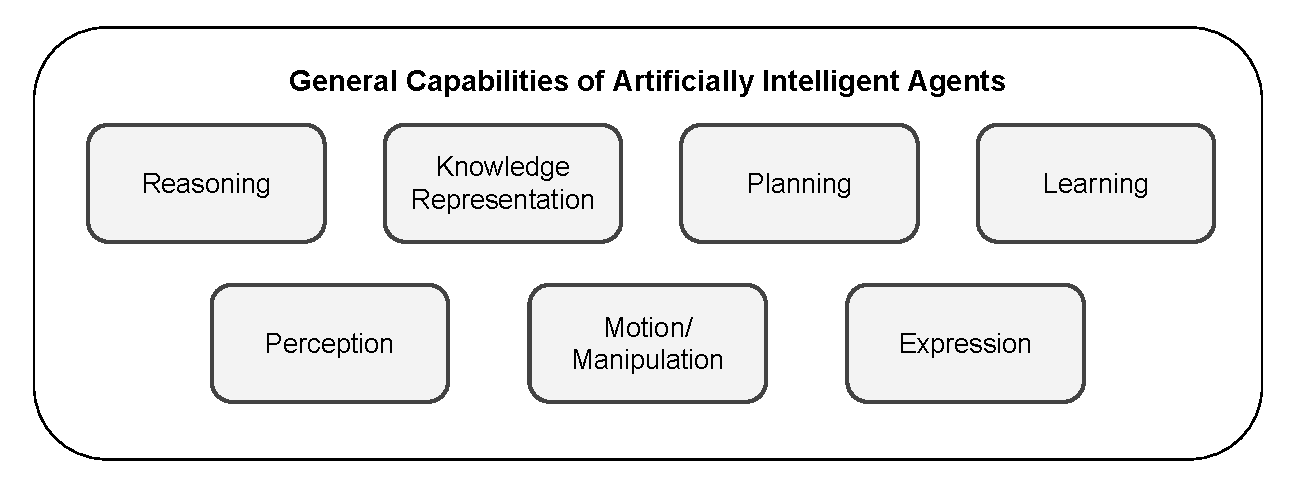
\includegraphics[width=0.9\textwidth]{Figures/AI_capabilities}
    	\caption{List of the capabilities of an artificial general intelligence. In this paper an AI is defined as a system that possesses at least one of the capabilities illustrated.}
        \label{fig:AIcapabilities}
    \end{figure}

    Concretely, the following systems currently exist and may possess the listed AI capabilities.
    
    \begin{enumerate}
         \item An unmanned aerial system (UAS) possesses the ability to plan, perceive, and move
         \item A personal assistant might be capable of interaction, learning, and reasoning.
         \item An image classifier might possess the capability to learn image classes from labeled examples and predict the class of never-before-seen new images.
         \item \textbf{More???}
     \end{enumerate}

\section{The Case for Human-AI Trust}
    Many would not be surprised to know that trust is critical in interpersonal relationships, and that it affects the dynamics of systems as simple as interpersonal relationships to more complicated ones such as financial markets \cite{Fukuyama1995-un} and governments. Consequently, researchers in psychology, sociology, and economics have historically sought to understand the fundamental principles of trust, each with the aim of understanding their field better \cite{Gambetta1988-pi}. Moral philosophers have also thought intently about the topic \cite{Baier1986-im}.

    In the early days of the internet there was a surge of interest in trust due to the appearance of e-commerce. Suddenly, a new forum for buying and selling wares and services appeared. How could relationships of trust be built between consumers and vendors in a new `online' ecosystem? Many researchers focused their efforts on exploring how to establish an ecosystem that would nurture the growth and prosperity of online businesses \cite{McKnight2001-fa}. This research is useful to those seeking to understand trust today because it focused on building such an ecosystem. Consequently the more practical understanding emerged that included some thoughts about how to affect trust. This survey will not exhaustively review the literature on trust; those interested might refer to the following works by \citet{McKnight2001-fa}, and \citet{Lewicki2006-hj}.

    Due to wide interest spanning many disciplines it is difficult, if not impossible, to write a succinct definition that would appease all interested parties. In their work relating to e-commerce \citet{McKnight2001-fa} reviewed much of the existing trust literature and attempted to distill the main concepts into a trust model that spanned disciplines. That model is shown, with some minor adaptations, in Figure \ref{fig:UserTrust}. Notice that the three main dimensions --- Dispositional Trust, Institutional Trust, and Interpersonal Trust --- are connected in such a way as to indicate some causal relationships between them. As trust cannot be directly measured there is no existing method with which to quantify the more detailed relationships between each of the dimensions of trust.

	\begin{figure}[htbp]
    	\centering
     	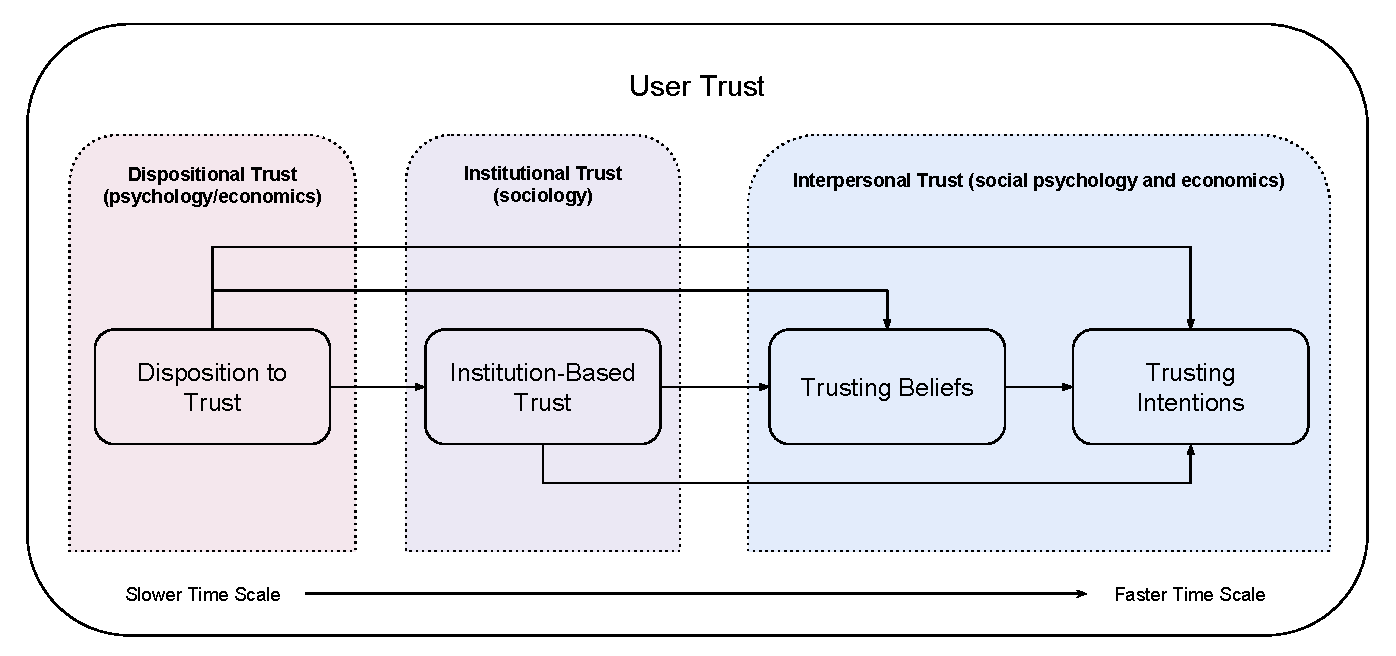
\includegraphics[width=0.9\textwidth]{Figures/UserTrust}
    	\caption{Interdisciplinary trust model proposed by \citet{McKnight2001-fa}. The three main categories are delineated and corresponding disciplines that are interested are listed within parentheses.}
        \label{fig:UserTrust}
    \end{figure}

    Something that is well accepted among researchers of all discplines is that trust results in some kind of behavior or action, which \citet{McKnight2001-fa} calls `trust-related behaviors' (TRBs). In the case of a human-autonomy relationship examples of TRBs might be the kinds of tasks the human user assigns to the autonomy, or whether the human will use a plan produced by the autonomy.

\section{Calibration of Trust-Related Behaviors}
    As yet, trust is not a quantity that can be directly measured. Rather, its relative magnitude must be observed through changes in TRBs. \citet{Parasuraman1997-co} were interested in understanding the use of automation which they defined as ``\ldots the execution by a machine agent (usually a computer) of a function that was previously carried out by a human''. Within this scope they define the following terms: a) \emph{misuse}, the overreliance on automation, b) \emph{disuse}, the underutilization of automation, and c) \emph{abuse}, inappropriate application of automation.

    Here it is proposed that, analogously, the definitions of \emph{misuse}, \emph{disuse}, and \emph{abuse} can apply to the relationship between humans and autonomy (where autonomy is defined as a system, such as an artificial agent with processing power possibly located on a physical robot, that is able to independently act in uncertain environments to accomplish a goal).
    
    To be more formal, let the total set of TRBs as $\mathcal{T}$. Then as subsets of $\mathcal{T}$ define the set of misue actions as $\mathcal{M}$, the set of disuse actions as $\mathcal{D}$, and the set of abuse actions as $\mathcal{A}$. Next, define the total set of innapropriate TRBs $\mathcal{I}$ as the union of $\mathcal{I} = \mathcal{M}\cup \mathcal{D}\cup\mathcal{A}$. Having defined the set of inappropriate actions, the set of appropriate TRBs can be defined as $\mathcal{U}$, the compliment of the set of inappropriate TRBs $\mathcal{U} = \mathcal{I}^\prime$. This is illustrated in Figure \ref{fig:appropriate_use}, where the set of appropriate actions $\mathcal{U}$ is the gray colored area (i.e. all TRBs \emph{not} in either of the three sets of inappropriate TRBs).
    
	\begin{figure}[htbp]
    	\centering
     	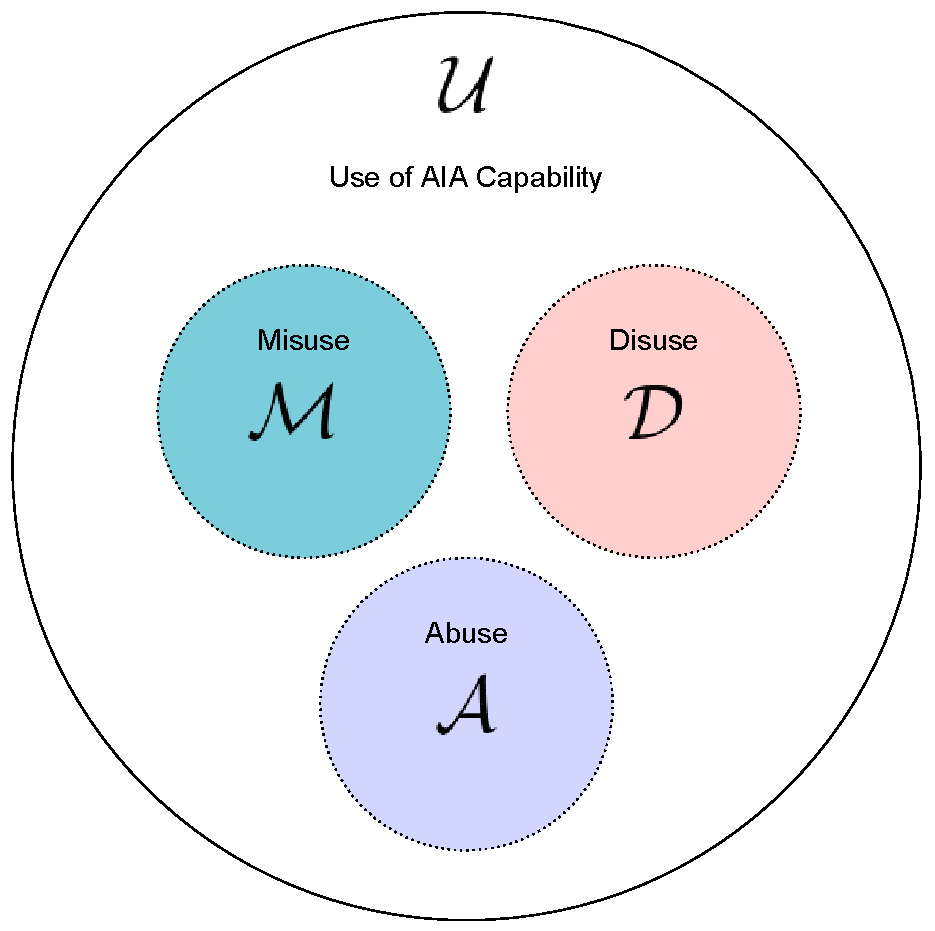
\includegraphics[width=0.4\textwidth]{Figures/misuse_disuse_abuse}
    	\caption{Graphic representing the total space of user actions, in which the inappropriate uses $\mathcal{M}$, $\mathcal{D}$, and $\mathcal{A}$ lie. The set of inappropriate uses $\mathcal{I}$ is the union of $\mathcal{M}$, $\mathcal{D}$, and $\mathcal{A}$. The appropriate set of actions $\mathcal{U}$ is the compliment of $\mathcal{I}$, or the part of $\mathcal{T}$ that does not include $\mathcal{I}$.}
        \label{fig:appropriate_use}
    \end{figure}
    
    In order to ensure that humans use autonomous systems appropriately it is critical that the user TRBs be calibrated to elicit behaviors that are within $\mathcal{U}$. This can be done by influencing the user trust.

    Generally trust between a human and AI could be depicted as in Figure \ref{fig:SimpleTrust_two_way}, where each has TRBs that must be calibrated, and each provides certain feedback, which will be called assurances, in order to do so. In a more simple scenario, where the AI implicitly trusts the human user the trust relationship can be depicted as shown in Figure \ref{fig:SimpleTrust_one_way}, where only the user has TRBs that are being calibrated.

	\begin{figure*}[htbp]
        \centering
        \begin{subfigure}[t]{0.48\textwidth}
            \centering
            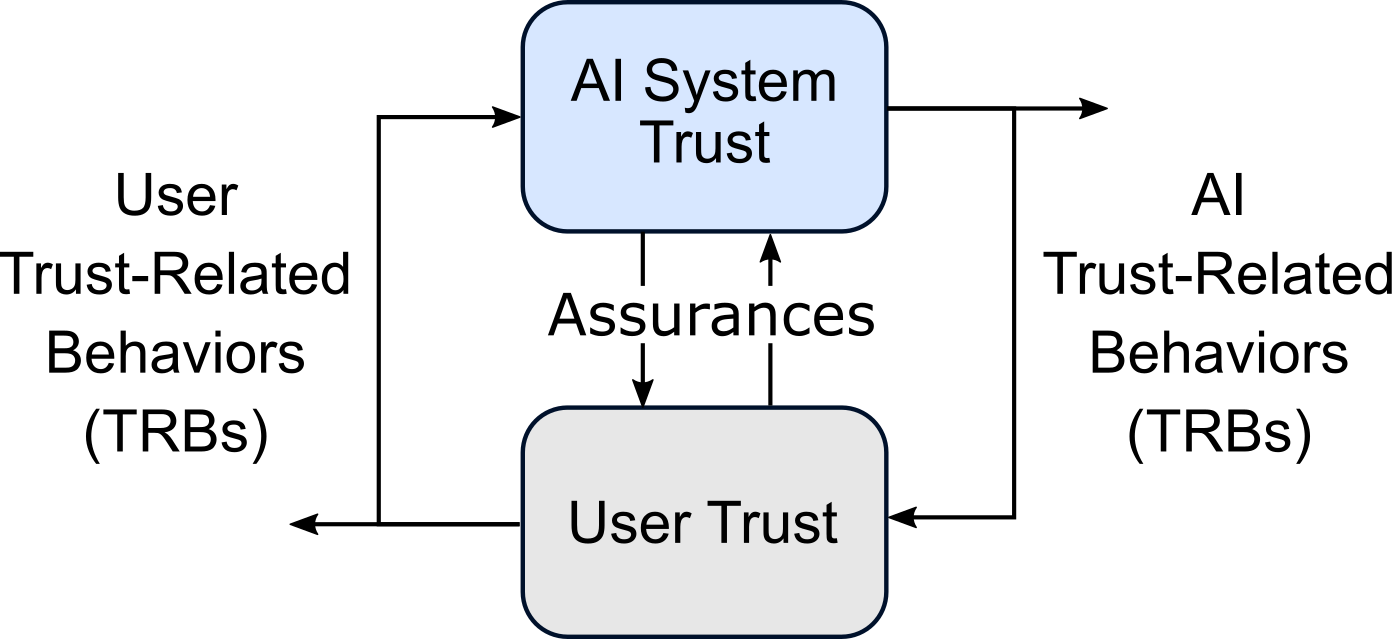
\includegraphics[width=0.95\textwidth]{Figures/SimpleTrust_two_way}
            \caption{Diagram showing a general case of a two-way trust relationship between an AI and a human. Arrows that are not connected to boxes represent some action outside of the trust loop.} 
            \label{fig:SimpleTrust_two_way}%
        \end{subfigure}
        \hfill
        \begin{subfigure}[t]{0.48\textwidth}
            \centering
            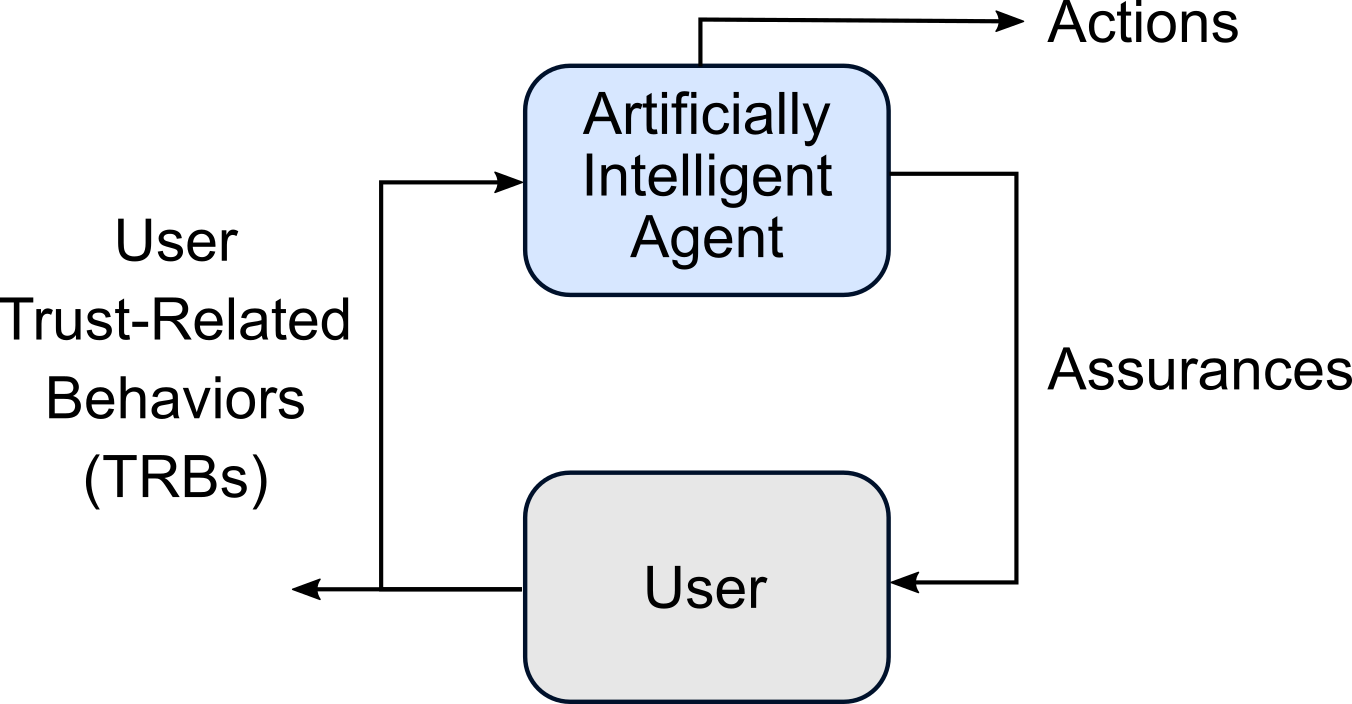
\includegraphics[width=0.95\textwidth]{Figures/SimpleTrust_one_way}
            \caption{Diagram illustrating a general one-way trust relationship between a human and an AI. In this case the AI has, what could be considered perfect trust in the user.}
            \label{fig:SimpleTrust_one_way}%
        \end{subfigure}
        \caption{Feedback Loops For One and Two-way human-AI Trust Relationships}
        \label{fig:SimpleTrust}
    \end{figure*}
    
    Figure \ref{fig:SimpleTrust_dist} serves as a simple example illustrating the possible disparity between the user TRB distribution and the appropriate TRB distribution. In this case assurances would be used to minimize the difference between the two distributions.

	\begin{figure}[htbp]
    	\centering
     	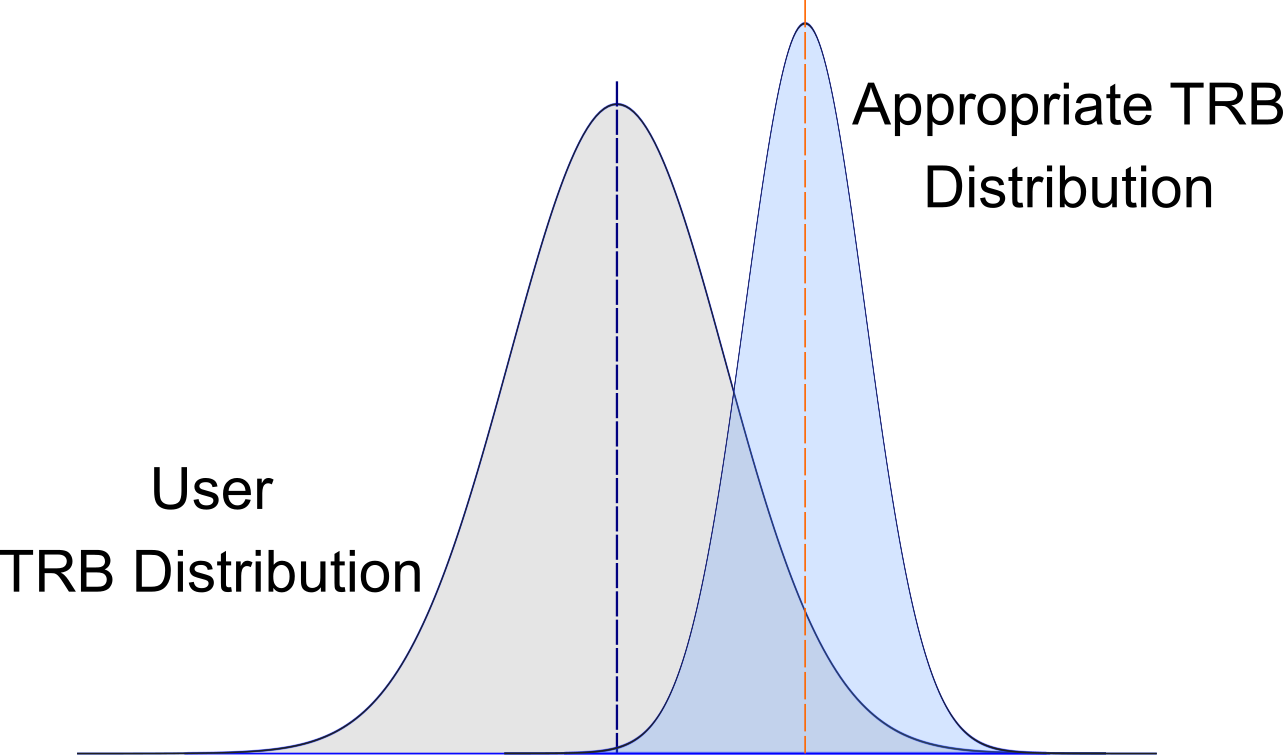
\includegraphics[width=0.4\textwidth]{Figures/SimpleTrust_dist.png}
    	\caption{Diagram illustrating the point that a hypothetical user TRB distribution might not match the appropriate TRB distribution. In this case the AI should provide assurances in order to minimize the difference between the two.}
        \label{fig:SimpleTrust_dist}
    \end{figure}


\section{Assurances}
    The term assurances was introduced in the previous section as the name by which feedback will be known in a human-AI trust relationship. A more detailed definition and discussion is merited.

    \citet{McKnight2001-fa} alludes to this kind of feedback in an e-commerce relationship as `Web Vendor Interventions' and mentions some possible actions that might be used in that specific application. They go as far as making a diagram that indicates that these interventions could affect the `Trusting Beliefs', `Trusting Intentions', and `Trust-Related Behaviors' (see Figure \ref{fig:UserTrust}).
    
    \citet{Lillard2016-yg} coined the term `assurances' as the ability of an autonomous system to affect the user's trust, and states that it is important to note that while generally the term assurance has a positive connotation; in this setting it must encompass both positive (increasing trust) and negative (decreasing trust) feedback.

    This work is meant to be related to that of \citet{Lillard2016-yg}, but more general. Here the assurance framework is set in a more general light, although with the goal of being applied in a very similar application. Instead of treating or at least inferring that the user-autonomy trust loop is very strict and well structured, and that user trust does not take into account the institutional component proposed by \citet{McKnight2001-fa}, we re-institute the notion of institutional trust into the human-autonomy relationships.

    Regarding the relationship with the work of \citet{McKnight2001-fa}, adopt the position that besides being applied to the e-commerce industry their trust model also applies to relationships between humans and autonomy (as in \citet{Lillard2016-yg}). However, it is argued that assurances cannot directly have an affect on the user TRBs. This premise is that no autonomy (or vendor) should be able to control the TRBs of a human.

	\begin{sidewaysfigure}[htbp]
        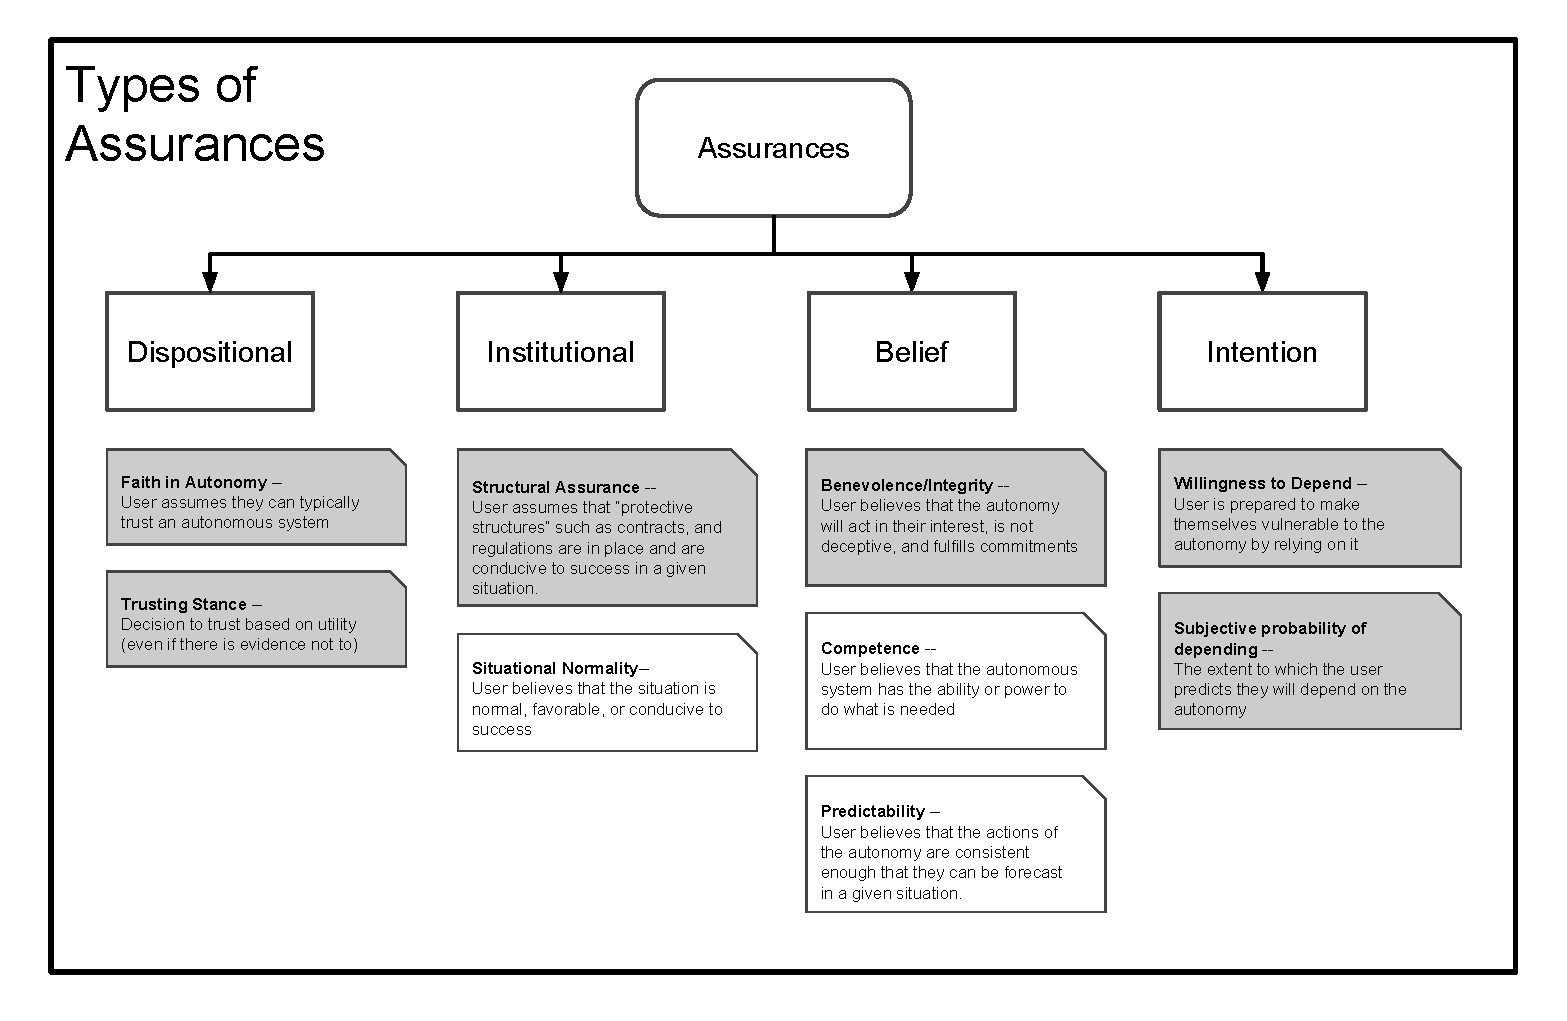
\includegraphics[width=8in]{Figures/Assurances.pdf}%
    	\caption{\textbf{Diagram delineating the possible classes of assurances, and suggesting those classes that directly apply in calibration of TRBs \ldots obviously needs to be finished \ldots}}
        \label{fig:Assurance_classes}
    \end{sidewaysfigure}

    Figure \ref{fig:Assurance_classes} shows the hierarchy of proposed assurance classes. The categories mirror those of the trust model proposed by \citet{McKnight2001-fa}, but with the emphasis on what an AI has the ability to influence. The colored boxes identify the different classes assurances. All classes are included here for completeness and generality. Although, due to practical limitations it might hypothetically possible for an AI to influence a persons general `Trusting stance' given enough time\footnote{One might imagine a AI that specifically speaks to the human about the benefits or drawbacks about trusting even though there might not be evidence to do so, similar to the role a counselor might play}, .

    Talk about the two classes of assurances: Passive and Active.

    \begin{description}
        \item [Passive:] Assurances that are not purposfully given by AI. Could be compared to non-verbal communication\ldots well not quite
        \begin{itemize}
            \item Such as success in completing the task (of course the autonomy wants to, but the outcome is independent).
            \item The way an autonomous vehicle looks when it is driving (something with weird driving habits for whatever reason might engender less trust). 
            \item 
        \end{itemize}
        \item [Active:] Assurances that are purposefully given by AI.
        \begin{itemize}
            \item Legible motion
            \item $R^2$
            \item Counter planning
            \item task similarity (to ideal task)
            \item etc.
        \end{itemize}
    \end{description}

    Each type of assurance can be given in passive or active ways. Perhaps they can be treated analogously to actions and words, specifically `actions speak louder than words' or `passive assurances speak louder than active ones'. The point is that actually doing something instead of just saying it will do a lot for bolstering trust. What is better saying: I can do this, or actually doing it?

    However, for the case of calibrating TRBs it is proposed that the classes should be constrained as shown in Figure \ref{fig:Assurance_classes}. An AI that is trying to calibrate the TRBs of a user (as opposed to just influencing them to its own benefit), should not actively try to convice the user that it should have faith in autonomy, or that it is benevolent, or that the institutional system should be trusted.

    Due to the nature of trust a single assurance might be targeted at influencing the competence dimension of trust, but it will likely also have affects on other dimensions. As an example an assurance aimed at influencing Predictability may also have an affect on the Probability of Depending.

    Besides being difficult to separate, each user is different. Thus no assurance will work identically when given to two separate users.

    \textbf{I am not sure how I want this argument to go, I want to highlight that it is theoretically possible to have some affect on each of these attributes, but that some are more practical. Two main things need to be considred 1) time-scale (how long will it take to make a noticeable change), and 2) what SHOULD be influenced in order to appropriately calibrate TRBs (it probably isn't acceptable to lie in order to manipulate a user's trust)?}
    

\section{Who cares?}
    Because everyone wants to trust their AIs, whether that be a single classification or regression algorithm, or a more interactive personal assistant that can understand language and communicate. Everyone wants to know how to trust these systems.  

    \paragraph{Why lay out AGI, when it doesn't exist yet?} Because this architecture is supposed to illustrate how the entire spectrum of AI from a single ML algorithm to an autonomous vehicle, to a full AGI operate on very similar grounds. That is that 

	\begin{sidewaysfigure}[htbp]
        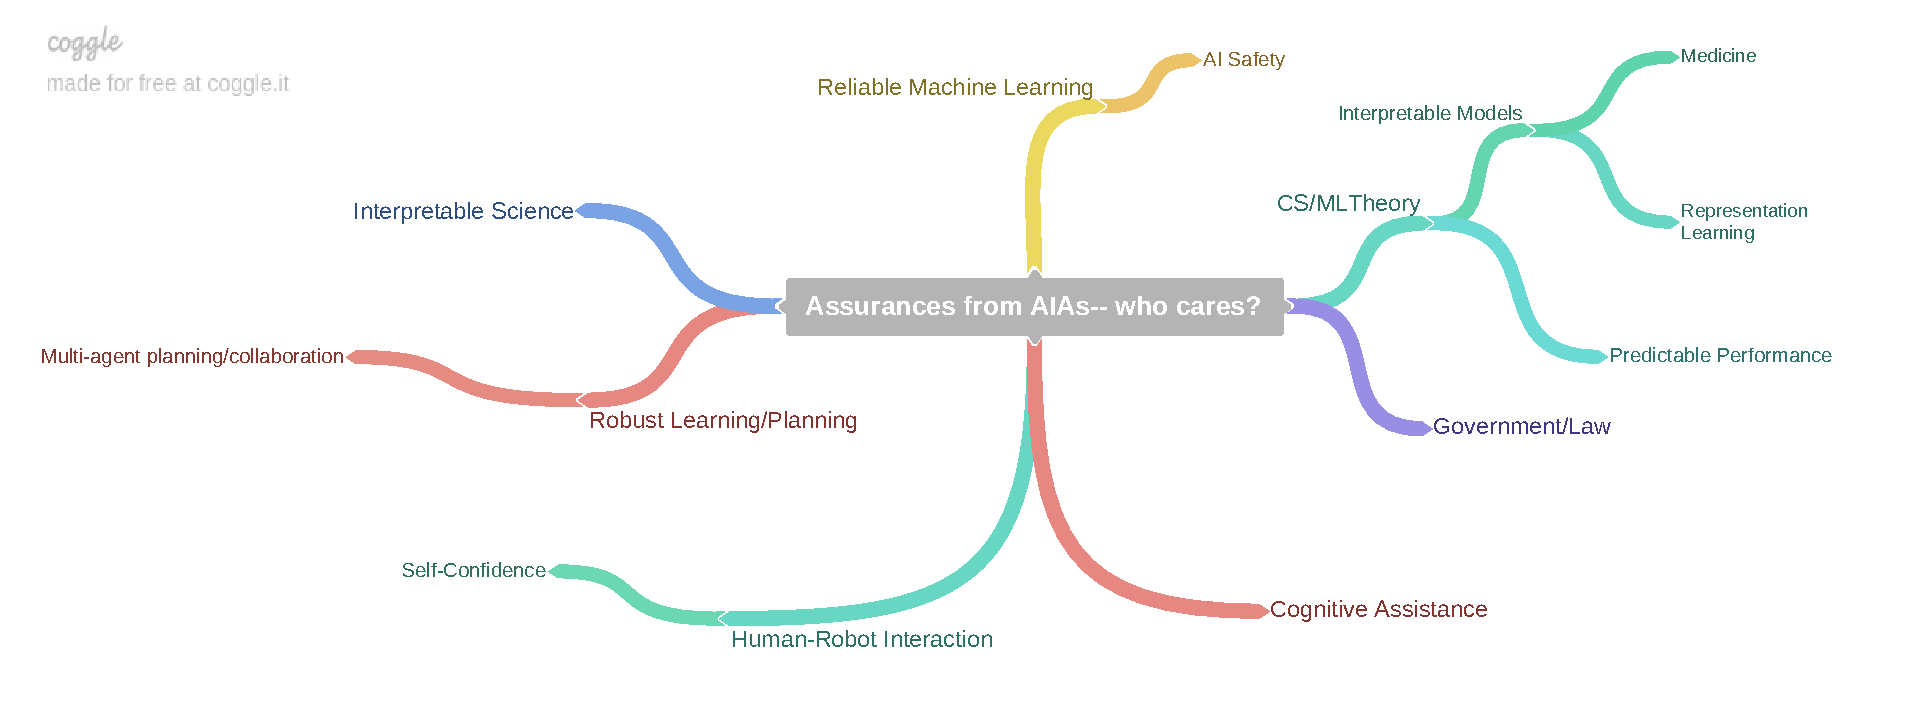
\includegraphics[width=8in]{Figures/WhoCares.pdf}%
    	\caption{A diagram showing some of the academic disciplines that want to trust AIs more fully}
        \label{fig:WhoCares}
    \end{sidewaysfigure}

    \paragraph{Science} Talk about why the science discplines care
    \paragraph{Robust Learning/Planning}
    \paragraph{HRI}
    \paragraph{Cognitive Assistance} 
    \paragraph{Government/Law} Regulations on the interpretability of certain algorithms, usage for assistants to lawyers.

    \textbf{Perhaps a table showing the field vs. the AI capability?}, this would help to illustrate the varying needs by fields. Perhaps highlight oversights?


% \input{samplebody-journals}

\bibliographystyle{ACM-Reference-Format}
\bibliography{References}
\end{document}
